\section{\textit{Minitwit's} Production Environment Dependencies}
\label{app:prod-deps}

\autoref{app:fig:bootstrap_deps} below illustrates the required dependencies to bootstrap a new production environment and destroy an existing production environment.

\begin{figure}[H]
    \centering
    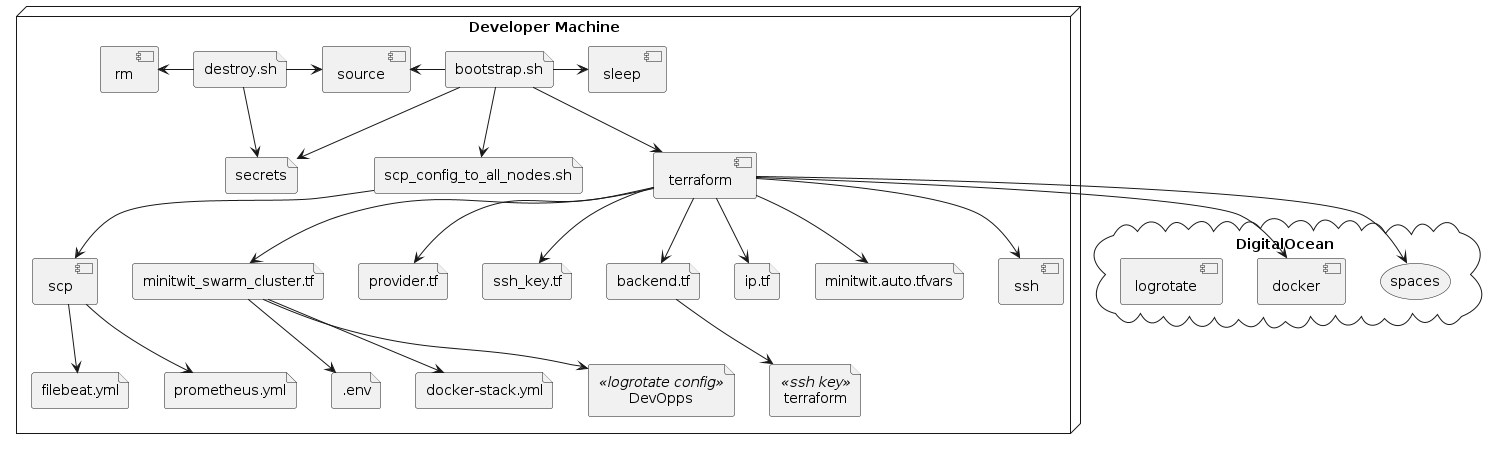
\includegraphics[width=\textwidth]{images/deps/bootstrap-deps.png}
    \caption{An illustration of the bootstrap and destroy script's dependencies}
    \label{app:fig:bootstrap_deps}
\end{figure}

\autoref{app:fig:deploy_deps} below shows the dependency of the deploy GitHub actions that is used to deploy new versions to production.

\begin{figure}[H]
    \centering
    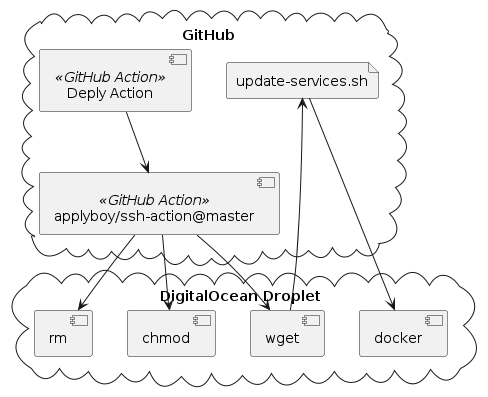
\includegraphics[width=\textwidth]{images/deps/do-deps.png}
    \caption{An illustration of the deployment dependencies}
    \label{app:fig:deploy_deps}
\end{figure}

In addition to the \textit{appleboy/ssh-action@master} GitHub action, the \textit{Build and Deploy} action depends on several more actions to build the \textit{Minitwit} system and package it using Docker containers.
They are listed below:
\begin{itemize}
    \item actions/checkout@v2
    \item bahmutov/npm-install@v1
    \item actions/upload-artifact@master
    \item actions/download-artifact@master
    \item docker/setup-qemu-action@v1
    \item docker/setup-buildx-action@v1
    \item docker/build-push-action@v2
\end{itemize}

Bootstrapping and destruction of production environments, as well as the \textit{Build and Deploy} GitHub action depend on a number of Debian packages. 
\autoref{app:tab:pkg_figs} lists  these packages and references the figure showing their dependency graphs.

\begin{table}[H]
    \centering
     \begin{tabular}{ |l|l| } 
        \hline
        Package & Dependency Graph \\
        \hline
        rm & No dependency info found \\
        \hline
        sleep & No dependency info found \\
        \hline
        terraform & No dependency info found \\
        \hline
        scp & No dependency info found \\
        \hline
        chmod & No dependency info found \\
        \hline
        ssh & \autoref{app:fig:ssh_dep_tree} \\
        \hline
        docker & \autoref{app:fig:docker_dep_tree} \\
        \hline
        logrotate & \autoref{app:fig:logrotate_dep_tree} \\
        \hline
        wget & \autoref{app:fig:wget_dep_tree} \\
        \hline
    \end{tabular}
    \caption{Debian packages and the corresponding dependency tree}
    \label{app:tab:pkg_figs}
\end{table}

\begin{figure}[H]
    \centering
    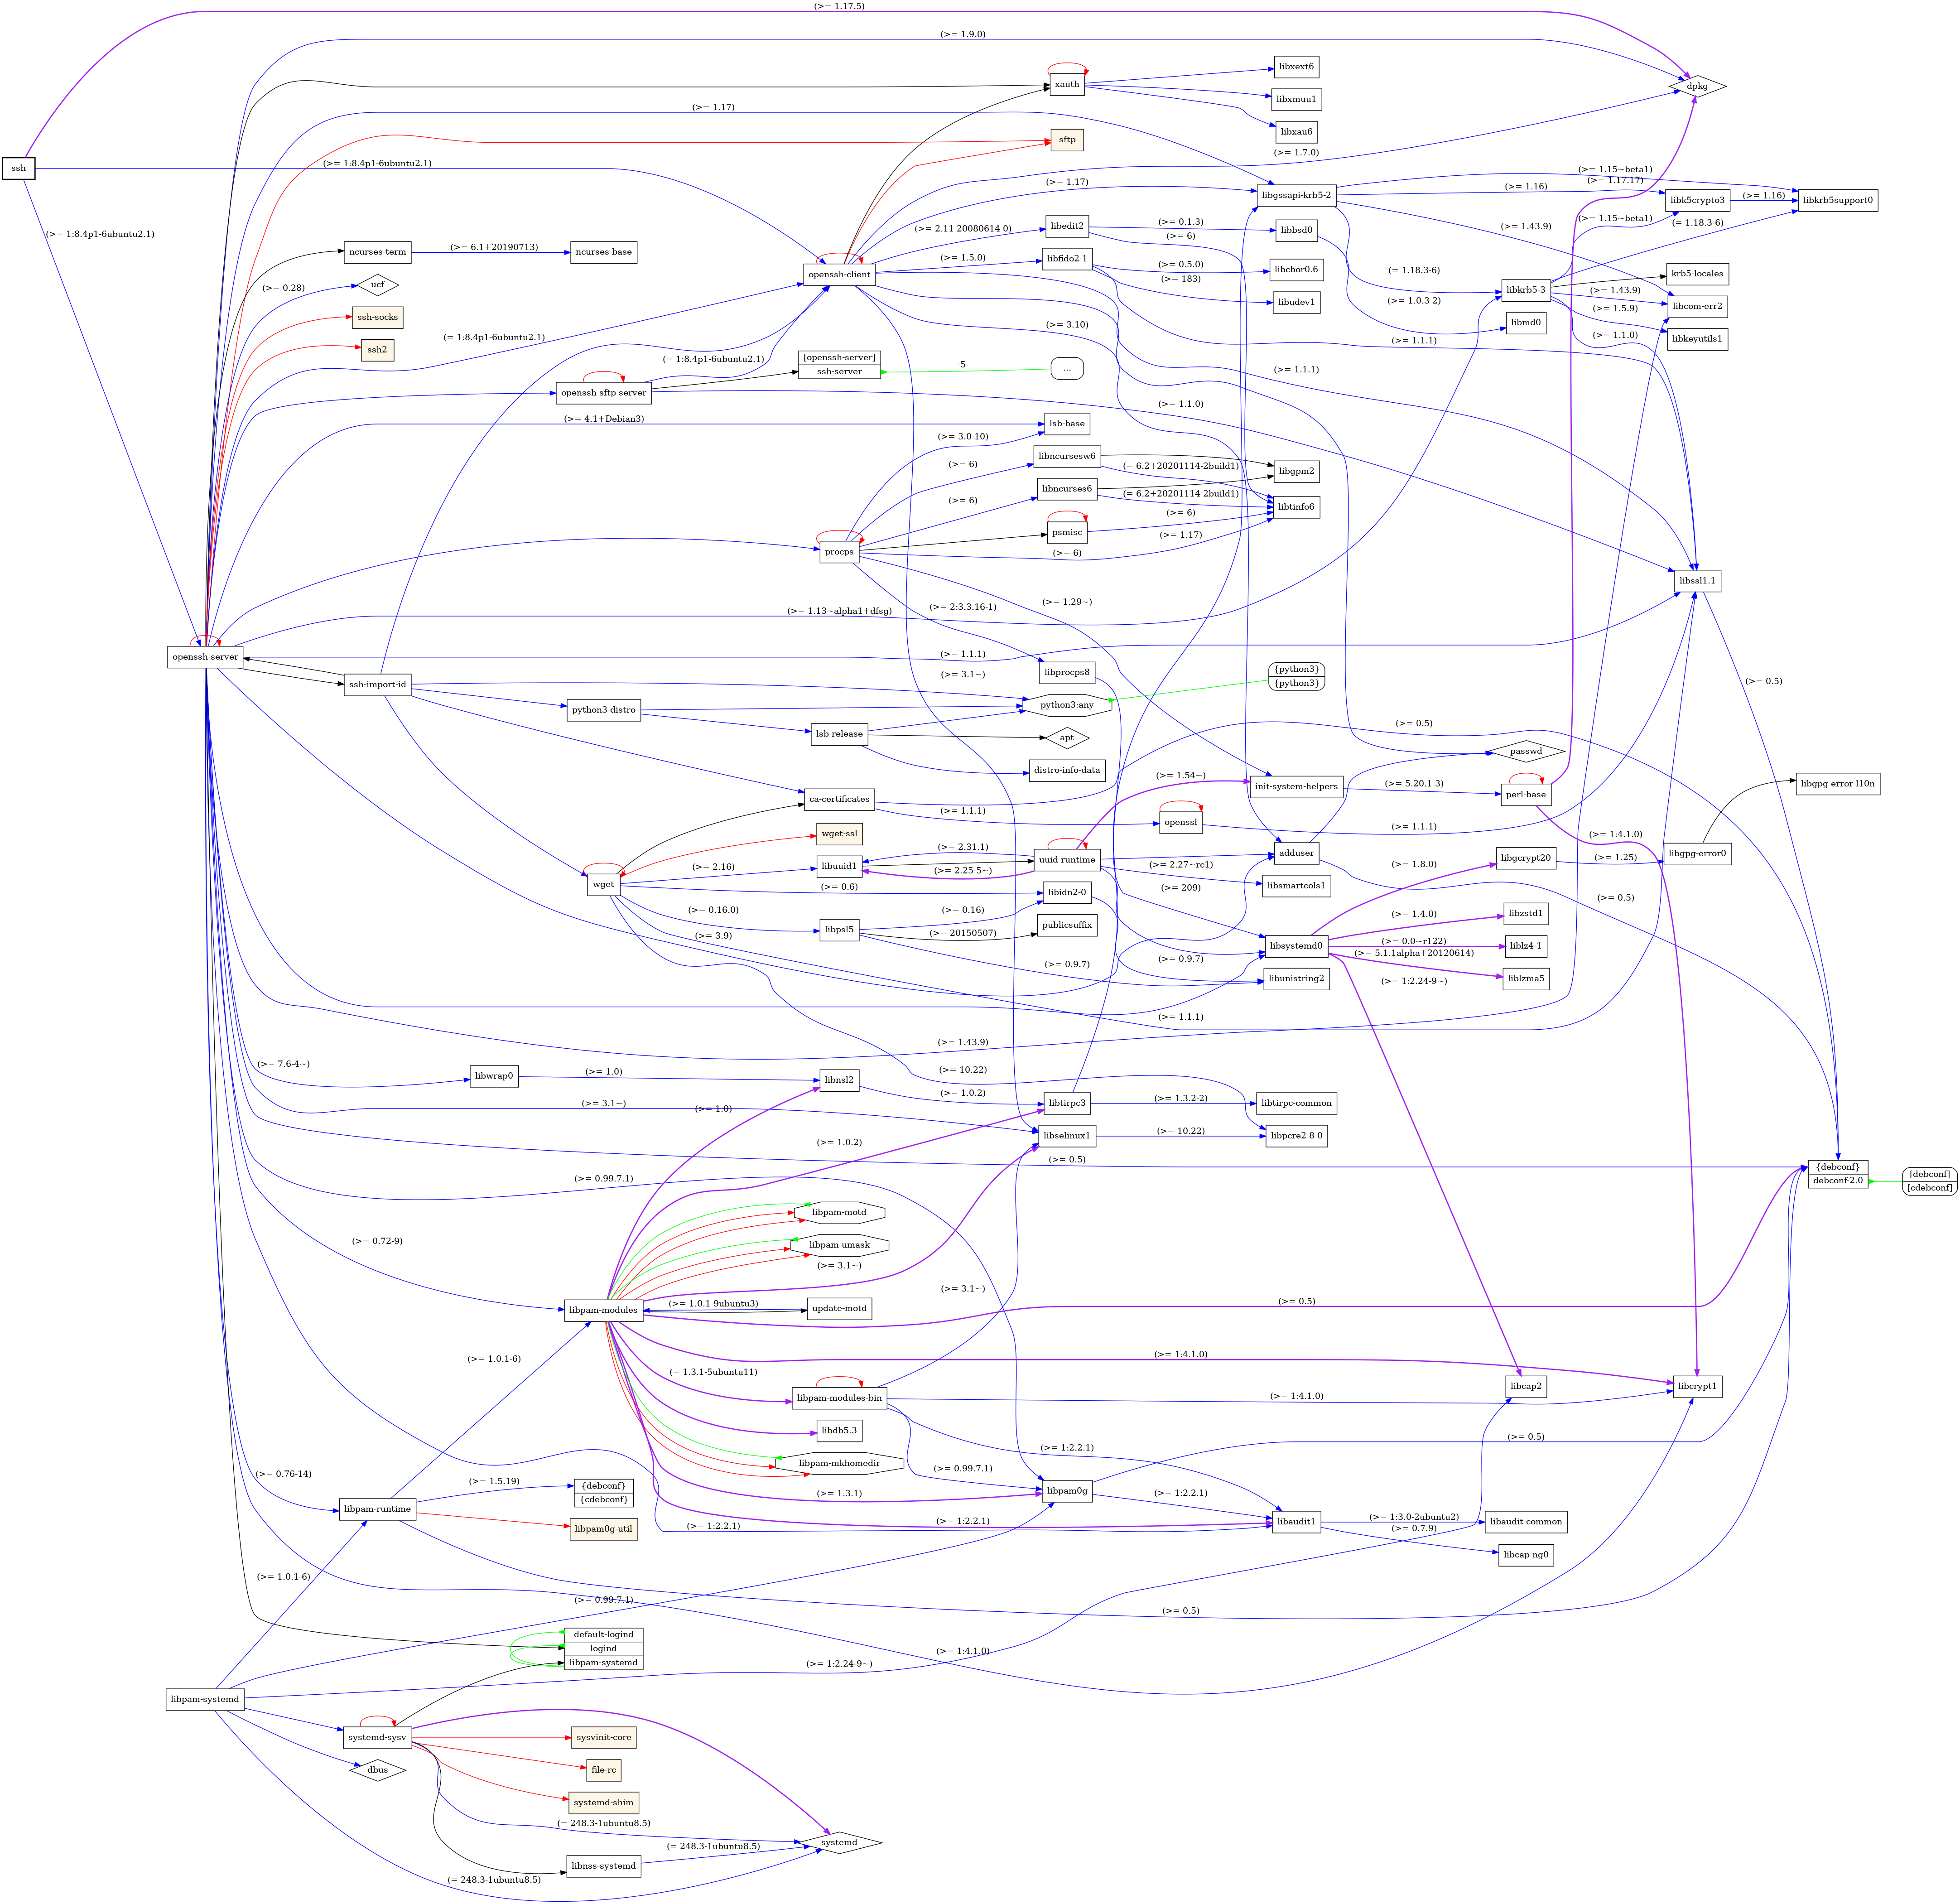
\includegraphics[width=\textwidth]{images/deps/ssh.png}
    \caption{SSH's Dependency Tree}
    \label{app:fig:ssh_dep_tree}
\end{figure}

\begin{figure}[H]
    \centering
    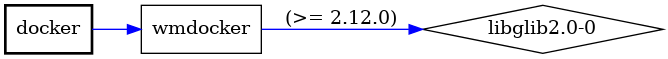
\includegraphics[width=\textwidth]{images/deps/docker.png}
    \caption{Docker's Dependency Tree}
    \label{app:fig:docker_dep_tree}
\end{figure}

\begin{figure}[H]
    \centering
    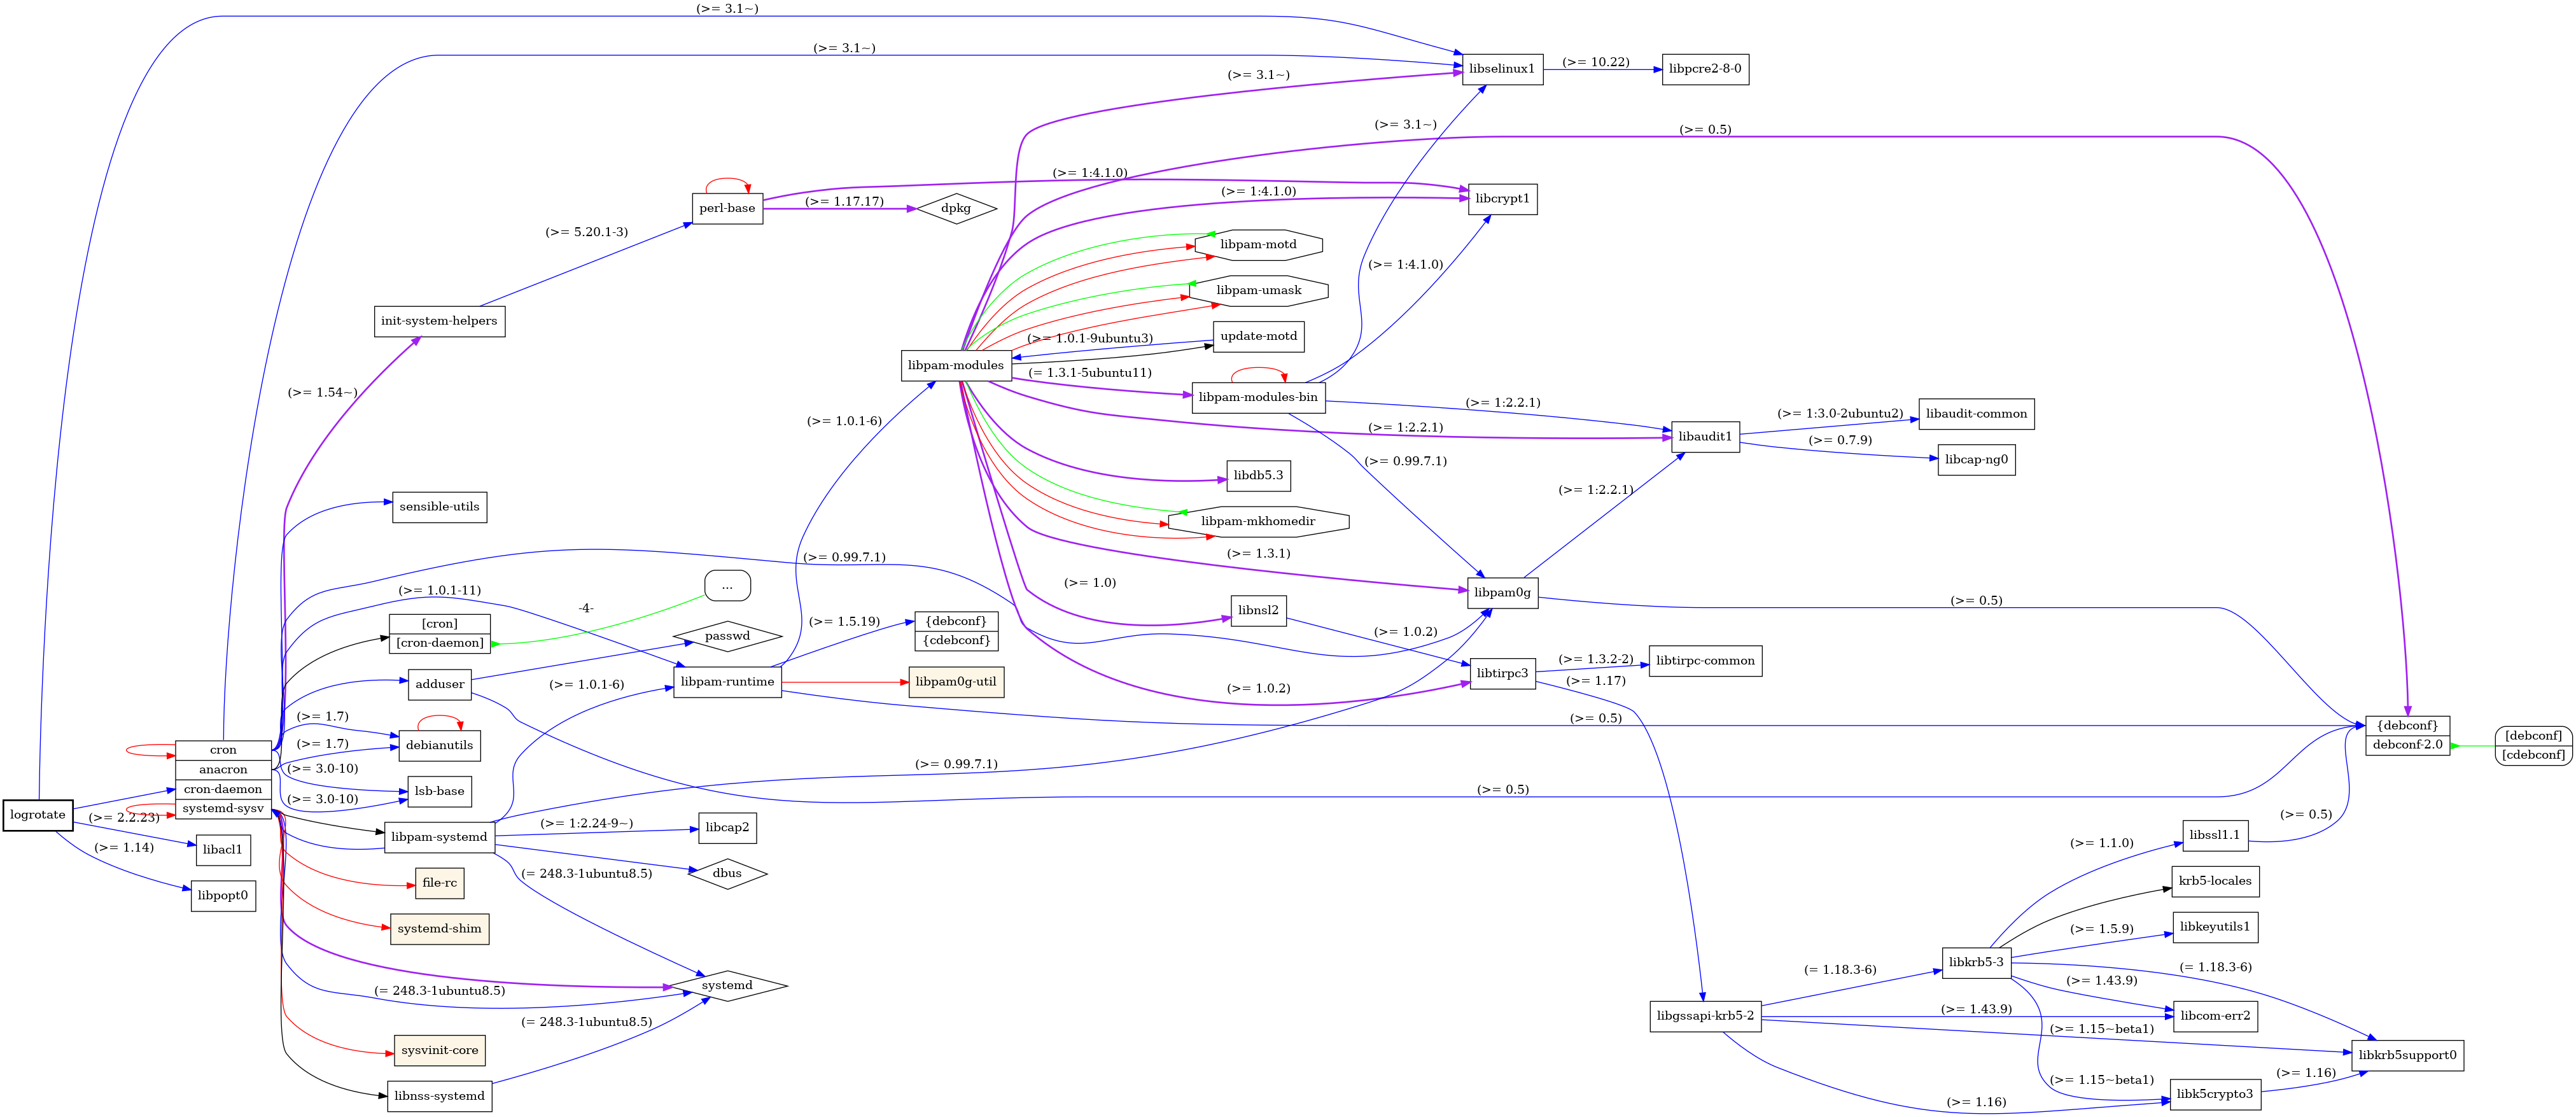
\includegraphics[width=\textwidth]{images/deps/logrotate.png}
    \caption{Logrotate's Dependency Tree}
    \label{app:fig:logrotate_dep_tree}
\end{figure}

\begin{figure}[H]
    \centering
    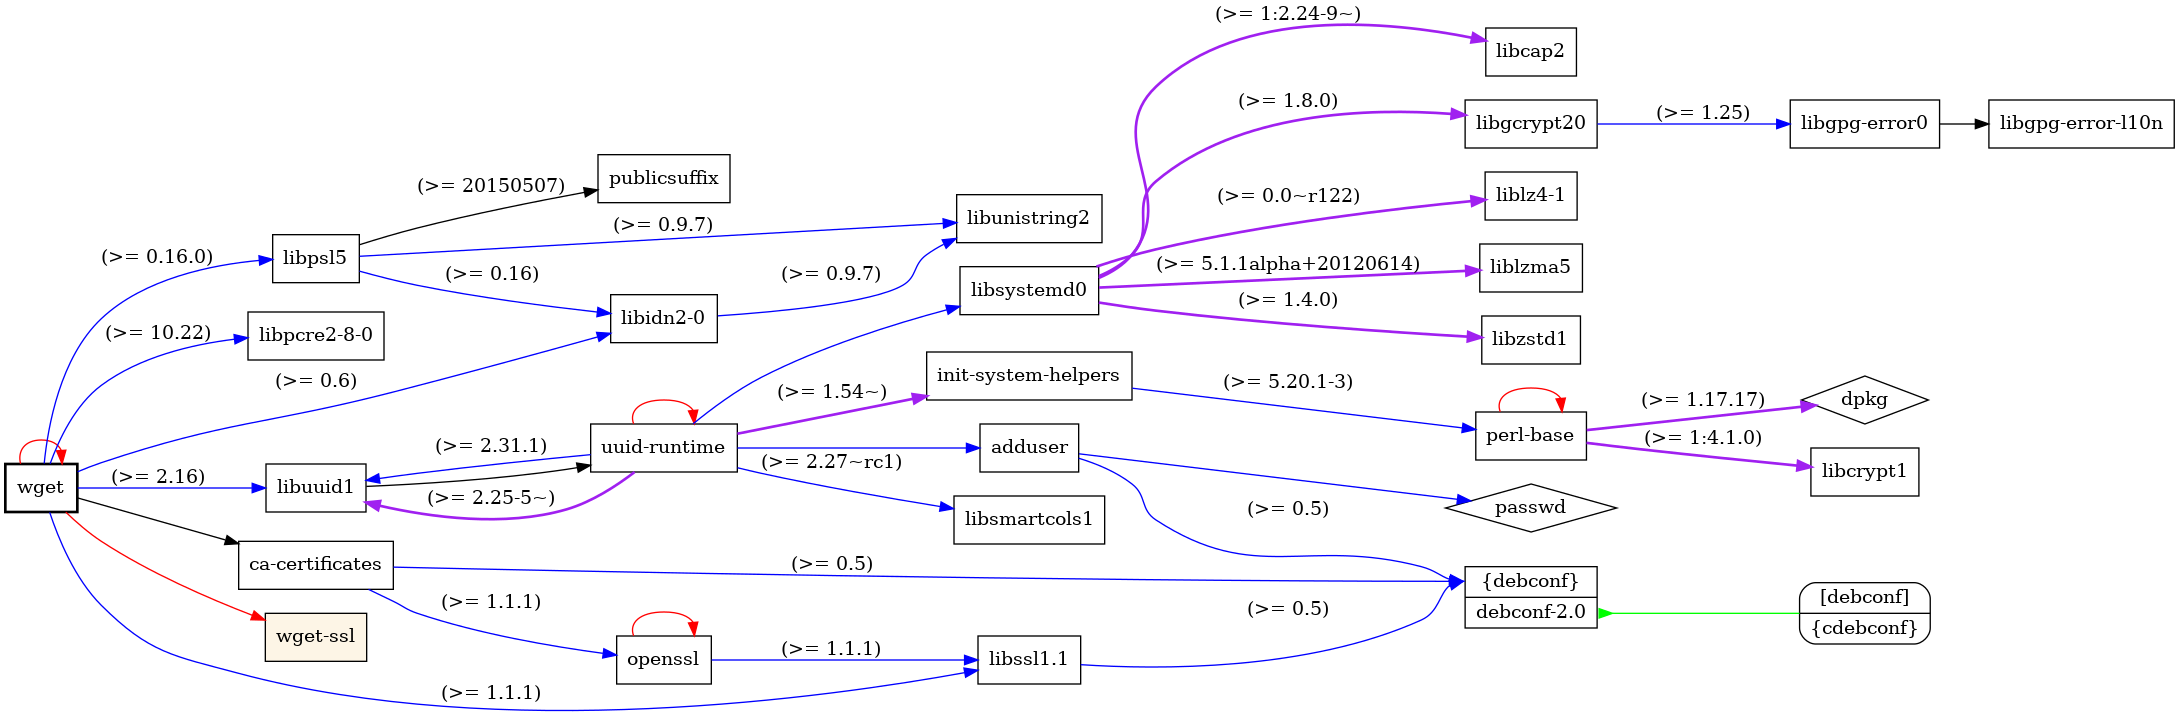
\includegraphics[width=\textwidth]{images/deps/wget.png}
    \caption{wget's Dependency Tree}
    \label{app:fig:wget_dep_tree}
\end{figure}
